\chapter{Bayesian probabilistic theory}

\label{ch:Bayesian}
In probabilistic theory, two main interpretations prevail: frequentist and Bayesian. The frequentist perspective views probabilities as the long-term frequencies observed in infinite trials. On the other hand, the Bayesian perspective links probability to uncertainty and information, diverging from repeated trials. 

Based on the quantity of accessible data, spanning from none to an infinite amount, diverse techniques can be employed:

\begin{itemize}[left=0pt]
 \item in cases where there is a lack of data to characterize the input parameters, a probabilistic model can be formulated solely based on expert judgment;
 \item when dealing with a substantial volume of data, one can fully leverage the tools of statistical inference, such as employing the method of moments \citep{wagner2020};
 \item when both expert judgment and very limited observations are available, Bayesian inference may be resorted to.
\end{itemize}

A notable benefit of the Bayesian interpretation lies in its ability to model events that lack long-term frequencies. Take, for example, the assessment of the probability of structural damage to a high-rise building, the collapse of a tunnel, or the occurrence of irreversible deformation in bridge piers. This event is anticipated to occur only a limited number of times over the structure's lifetime and is not expected to happen repeatedly. Subsequently, it is important to quantify our uncertainty regarding this event and implement appropriate measures (see chapter \ref{UQ} and chapter \ref{Work_Plan}).

Since data collection is inherently constrained during the progression of most engineering projects (e.g., geotechnical problems), Bayesian theory stands out as a highly effective method. Therefore, this thesis exclusively explores Bayesian methods next, while detailed information on frequentist approaches can be found in \cite{murphy2012}.






\section{Bayesian inference}

When dealing with a limited number of data points, direct statistical estimation becomes unreliable due to substantial statistical uncertainty in the sample estimates. In this context, Bayesian inference provides a solution by integrating prior knowledge on parameters with a small set of observed data points. Operating in this fully probabilistic setting, all unknowns are treated as random vectors. Distribution parameters can be denoted by $\boldsymbol{x}$ as realisations of the random vector $\boldsymbol{X}:\Omega \rightarrow \mathcal{D}_{\boldsymbol{X}}$. \textit{Quantities of interest} gathered from output are gathered in a vector $\boldsymbol{y} \in \mathbb{R}^{N_{\rm{out}}}$. The joint probability distribution of the combined random vector $(\boldsymbol{X},\boldsymbol{Y}):\Omega \rightarrow \mathcal{D}_{\boldsymbol{X}} \times {D}_{\boldsymbol{Y}}$ is represented by $\pi(\boldsymbol{x};\boldsymbol{y})$. Leveraging the fundamental \textit{sum rule} and \textit{product rule} in probabilistic theory, the \acrfull{PDF} of the parameters $\boldsymbol{x}$ and the data $\boldsymbol{y}$ can be expressed as
\begin{equation}
\pi(\boldsymbol{x}|\boldsymbol{y}) = \frac{{\mathcal{L}(\boldsymbol{x};\boldsymbol{y}) \cdot \pi(\boldsymbol{x})}}{{\pi(\boldsymbol{y})}} \label{equation Bayes}
\end{equation}
which is also known as \textit{Bayes' theorem} or \textit{Bayes' rule}. In Bayesian terminology, this distribution $\pi(\boldsymbol{x}|\boldsymbol{y})$ is called the posterior distribution and it is calculated by prior $\pi(\boldsymbol{x})$, likelihood $\mathcal{L}(\boldsymbol{x};\boldsymbol{y})\stackrel{\mathrm{def}}{=}\pi(\boldsymbol{y}|\boldsymbol{x})$
and the evidence $\pi(\boldsymbol{y})$. These definitions of the likelihood function and evidence strictly hold only for a single data point $\mathcal{Y}=\{\boldsymbol{y} \}$, but can be generalised to multiple data points easily $\mathcal{Y} \stackrel{\mathrm{def}}{=} \{{\boldsymbol{y}^{(1)}},\cdots,{\boldsymbol{y}^{(N)}}\}$. These terms in \cref{equation Bayes} have practical significance that we will briefly summarise next.
\begin{itemize}[left=0pt]
    \item \textcolor{blue}{Prior $\pi(\boldsymbol{x})$}: In the Bayesian paradigm, before considering the data, the parameters $\boldsymbol{x}$ are treated as realisations derived from a random vector $\boldsymbol{X}$ presumed to adhere to the so-called prior distribution.


    \item \textcolor{blue}{Likelihood function $\mathcal{L}(\boldsymbol{x};\mathcal{Y})$}: The likelihood function gauges the adequacy of the specified parametric distribution $\pi(\mathcal{Y}|\boldsymbol{x})$ describes the data. In most engineering cases, input parameters $\boldsymbol{x}$ are not measurable directly. To evaluate the likelihood $\mathcal{L}(\boldsymbol{x};\mathcal{Y})$, some ingredients are needed: a forward model $\mathcal{M}$, inferred input parameters $\boldsymbol{x} \in\mathcal{D}_{\boldsymbol{X}}$, and a collection of experimental data $\mathcal{Y}$.
The forward model $\boldsymbol{x} \rightarrow \boldsymbol{\mathcal{M}}(\boldsymbol{x})$ is a representation of a physical system under consideration. Thus, to establish a connection between the observations $\mathcal{Y}$ and model predictions, we introduce a \textit{discrepancy term} $\boldsymbol{\varepsilon}$ and consider the following well-established format as:
\begin{equation}
        \label{eq: discrepancy term}
        \boldsymbol{y} = \mathcal{M}(\boldsymbol{x}) + \boldsymbol{\varepsilon}
    \end{equation}
where $\boldsymbol{\varepsilon} \in \mathbb{R}^{N_{\rm{out}}}$ denotes the difference between the observation $\boldsymbol{y}$ and the prediction $\mathcal{M}(\boldsymbol{x})$. For the sake of simplicity, we consider it as an additive \textit{Gaussian discrepancy} with zero mean and a covariance matrix $\boldsymbol{\Sigma}$ in this introduction:
\begin{equation}
            \label{eq: Gaussian discrepancy}
            \boldsymbol{\varepsilon} \in \mathcal{N}(\varepsilon|\boldsymbol{0},\boldsymbol{\Sigma})
        \end{equation}
If there are $N$ independent measurements $\boldsymbol{y_{i}}$ collected in the dataset $\mathcal{Y} \stackrel{\mathrm{def}}{=} \{{\boldsymbol{y}_{(1)}},\cdots,{\boldsymbol{y}_{(N)}}\}$, the likelihood can expressed as follows:
\begin{equation}        
        \label{eq: Likelihood function}
        \begin{aligned}
         \mathcal{L}(\boldsymbol{x};\mathcal{Y}) =& \prod_{i=1}^{N} N(\boldsymbol{y_{i}}|\mathcal{M}(\boldsymbol{x}),\boldsymbol{\Sigma}) \\
         =& \prod_{i=1}^{N}\frac{1}{\sqrt{(2 \pi)^{N_{\rm{out}}}{\rm{det}} 
         (\boldsymbol{\Sigma})}}\exp\left(-\frac{1}{2}\left(\boldsymbol{y_i} - \mathcal{M}(\boldsymbol{x})\right)^{\mathsf{T}} \boldsymbol{\Sigma}^{-1}\left(\boldsymbol{y_i} - \mathcal{M}(\boldsymbol{x})\right)\right) 
        \end{aligned}
        \end{equation} 
It is noted that simple Gaussian discrepancy assumption is only one out of many possible models. In a more general setting, other distributions for the discrepancy are used as well \citep{UQdoc}. Due to the widespread used of the additive Gaussian models in engineering disciplines, this thesis is limited to Gaussian type. 
    \item \textcolor{blue}{Evidence $\pi(\mathcal{Y})$}: In Bayesian inference, $\pi(\mathcal{Y})$ is commonly regarded as a normalization factor, ensuring that the posterior \acrshort{PDF} can be integrated to one:
\begin{equation}
        \label{eq: evidence}
        \pi(\mathcal{Y}) \stackrel{\rm{def}}{=} \int_{\mathcal{D}_{\boldsymbol{X}}} 
        {\mathcal{L}(\boldsymbol{x};\mathcal{Y}) \pi(\boldsymbol{x})}
        {\rm{d}} \boldsymbol{x}
    \end{equation}
\end{itemize}

A schematic Bayesian inference in two dimensional space is displayed in \cref{fig: BI_2D}. The plots show the various elements of the Bayesian inference procedure in the parameter and data spaces. We can see that in the parameter space, with new experimental data comes in, the posterior is more concentrated than the prior distribution. 
\begin{figure}[htbp]
    \centering
    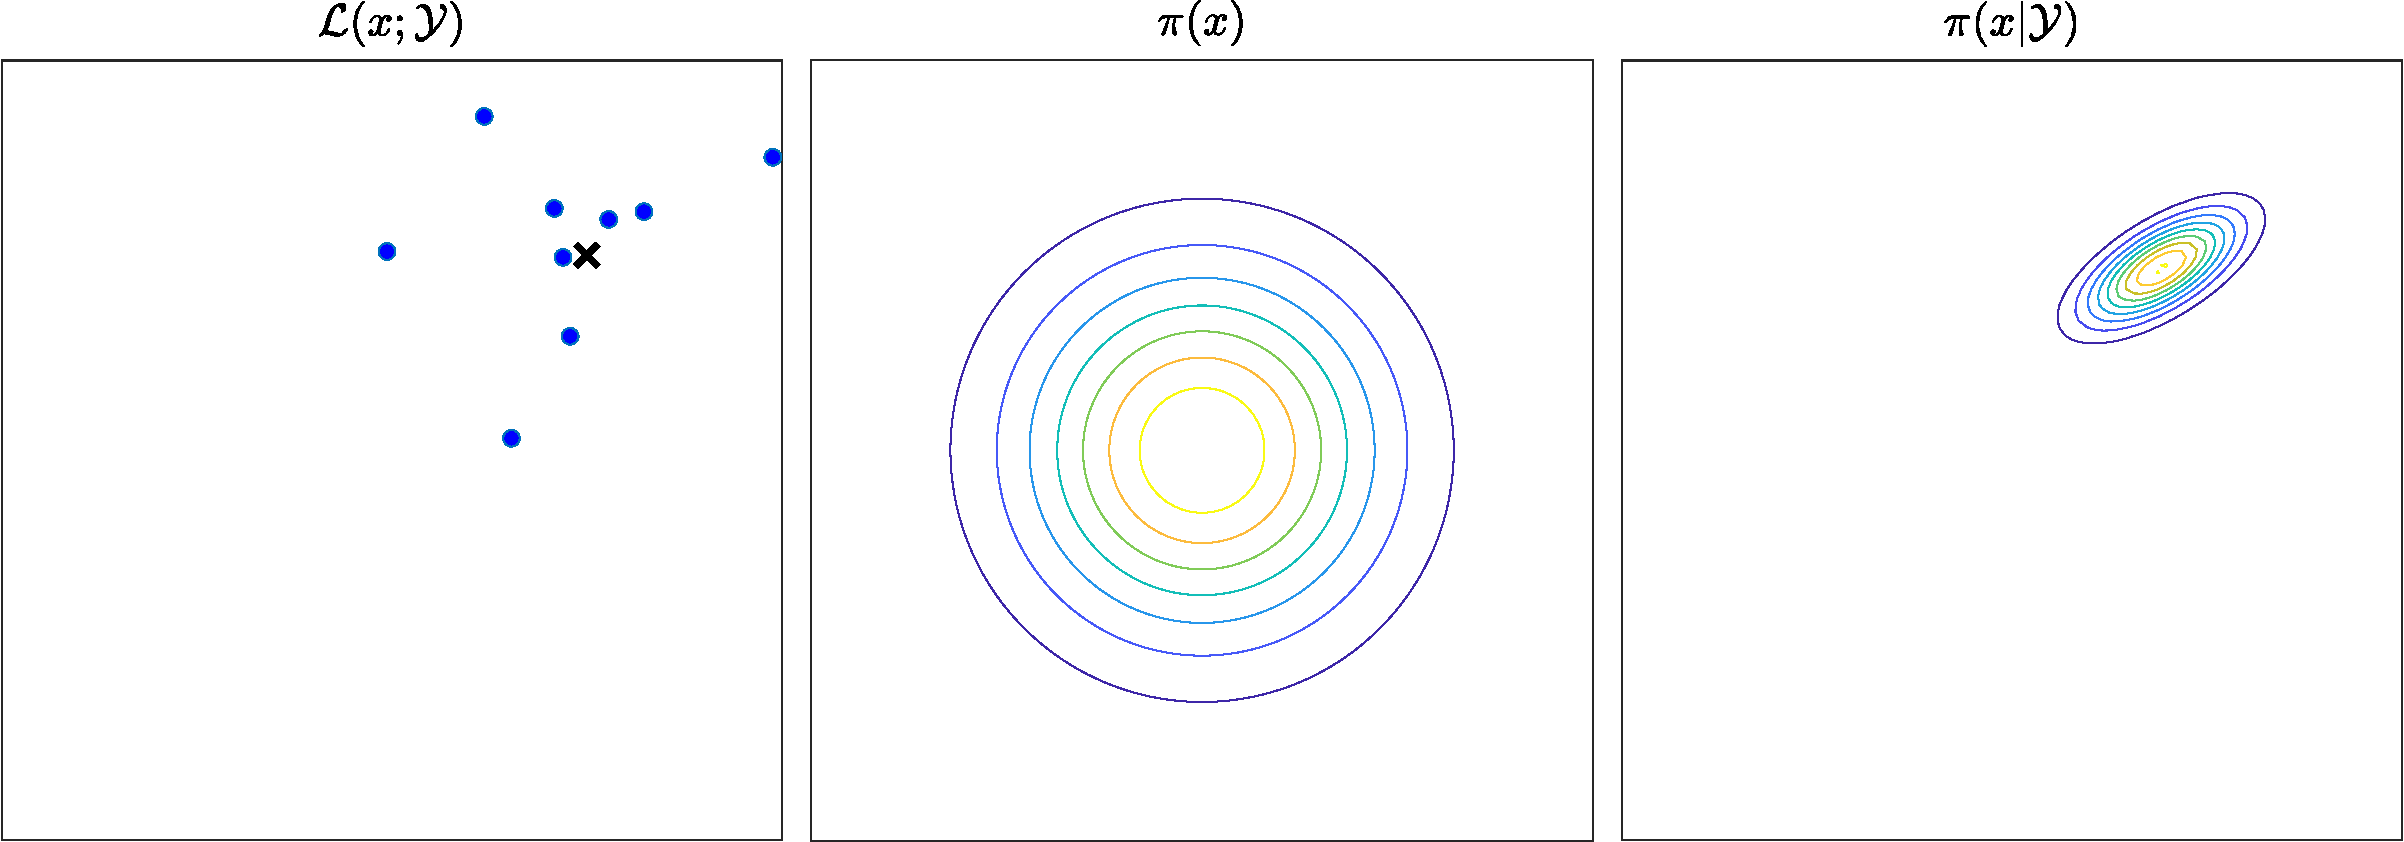
\includegraphics[width = 140mm]{Figures/figure-BI_2D.pdf}
    \caption{An Bayesian inference example in 2D space}
    \label{fig: BI_2D}
\end{figure}
\section{Posterior quantities of interest}
Under the Bayesian paradigm, the posterior distribution $\pi(\boldsymbol{x}|\mathcal{Y})$ is the solution of the inverse problem. However, in practice it can also serve as an intermediate result that is further processed for interpretation or prediction purpose. Furthermore, the full distribution can contain too much information to allow statements about the inferred parameters. Therefore, it is common to process the posterior and extract certain quantities of interest that summarize the inversion results more concisely.

\subsubsection{Point estimate}

In many applications, one is only interested in a single parameter, i.e., the one that characterise the inversion most suitably. The two most common \textit{point estimation} methods are the \textit{posterior mean} $\boldsymbol{x}^{\rm{mean}}$ and \acrfull{MAP}. The $\boldsymbol{x}^{\rm{mean}}$ is given as:
\begin{equation}
    \label{eq: posterior mean}
    \boldsymbol{x}^{\rm{mean}} = \mathbb{E}[\boldsymbol{X}|\mathcal{Y}] = \int_{\mathcal{D}_{\boldsymbol{X}|\mathcal{Y}}} 
    \boldsymbol{x} \pi(\boldsymbol{x}|\mathcal{Y}) {\rm{d}} \boldsymbol{x}  
\end{equation}
It reflects what we expect the parameter value to be after the inference. The \acrshort{MAP} parameter, on the other hand, is the one maximises the posterior:
\begin{equation}
    \label{eq: MAP}
    \begin{aligned}
       \boldsymbol{x}^{\rm{MAP}} &= \mathop{\arg\max}\limits_{\boldsymbol{x} \in \mathcal{D}_{\boldsymbol{X}}}
    \pi(\boldsymbol{x}|\mathcal{Y}) \\
    &=\mathop{\arg\max}\limits_{\boldsymbol{x} \in \mathcal{D}_{\boldsymbol{X}}}
   {\mathcal{L}(\boldsymbol{x};\mathcal{Y}) \pi(\boldsymbol{x})}     
    \end{aligned}
\end{equation}
where the evidence constant $\pi(\mathcal{Y})$ was omitted. The \acrshort{MAP} point corresponds to the most likely value of the input parameters. It is closely related to the \acrfull{ML} point that is defined as 
\begin{equation}
    \label{eq: MLE}
    \boldsymbol{x}^{\rm{ML}}  = \mathop{\arg\max}\limits_{\boldsymbol{x} \in \mathcal{D}_{\boldsymbol{X}}}
   {\mathcal{L}(\boldsymbol{x};\mathcal{Y})}
\end{equation}
for which the forward model $\mathcal{M}$ produces the best agreement with the available data. Unlike the \acrshort{ML}, the \acrshort{MAP} point considers the prior information. The difference is typically larger in the case of little data, where the regularisation effect of the prior distribution is stronger. In case of uniform priors, the two are equal, provided that the \acrshort{ML} point does not lie outside the prior support.

\subsubsection{\textit{Posterior moments} and \textit{covariance}}
Choices for the point estimation above disregards the estimation uncertainty in the parameters. Therefore, to more comprehensively characterise the posterior distribution and investigate the calibration, it is useful to compute the second $\textit{posterior moments}$ and the $\textit{covariance}$. They are summarised in the $\textit{posterior covariance matrix}$ $\boldsymbol{C} \in \mathbb{R}^{M \times M}$ with entries:
\begin{equation}
    \label{eq: COV}
    \begin{aligned}
    \boldsymbol{C}  &= {\rm{Cov}}[\boldsymbol{X}|\mathcal{Y}] \\
            &=\int_{\mathcal{D}_{\boldsymbol{X}}} 
            (\boldsymbol{x} - \mathbb{E}[\boldsymbol{X}|\mathcal{Y}])(\boldsymbol{x} - \mathbb{E}[\boldsymbol{X}|\mathcal{Y}])^{\mathsf{T}} \pi(\boldsymbol{x}|\mathcal{Y}) {\rm{d}} \boldsymbol{x} 
    \end{aligned}  
\end{equation}
\begin{figure}[htbp]
    \centering
    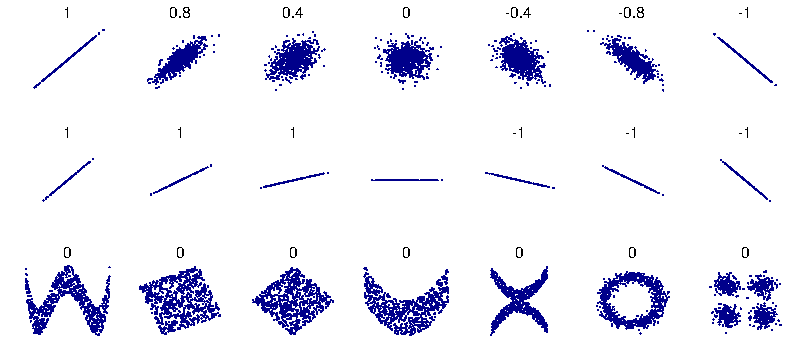
\includegraphics[width = 140mm]{Figures/figure-COV.pdf}
\caption{Example sets of ($x,y$) points with different \acrshort{COV} from \cite{Wikipedia}}
    \label{fig: COV}
\end{figure}
As the full posterior distribution is an \textit{M}-dimensional object, which is inherently difficult to comprehend, one is typically also interested in the \textit{posterior marginals} and \textit{copula dependence}. The marginalised random variable $X_{i}|\mathcal{Y}$ is given by (see \cref{eq: Margin_Post}):
\begin{equation}
    \label{eq: Margin_Post}
    \pi(x_{i}|\mathcal{Y}) = \int_{\mathcal{D}_{\boldsymbol{X}_{\rm{\boldsymbol{v}}}}}
          \pi(\boldsymbol{x}|\mathcal{Y}){\rm{d}} \boldsymbol{x_{\rm{\boldsymbol{v}}}}, {\rm{with}} \ \boldsymbol{\mathrm{v}} = \{1,\cdots,M\} \backslash i  
\end{equation}
This univariate \acrshort{PDF} can be integrated to obtain the corresponding \acrfull{CDF} which may then be used to define \acrfull{CI} on the calibrated parameters by means of quantiles. \textit{Copula dependence} can be inferred easily from the joint \acrshort{PDF} as $\boldsymbol{C}$. Different types of \acrshort{COV} can be seen in \cref{fig: COV}.

\subsubsection{Predictive distribution}
Next, to evaluate the predictive prowess of the model, the Bayesian inference framework offers the possibility to compute \textit{predictive distributions}. Using previously defined discrepancy model from \cref{eq: Gaussian discrepancy} and \cref{eq: discrepancy term}, the \textit{prior predictive} distribution can be represented as:
\begin{equation}
    \label{eq: prior predictive}
    \pi(\boldsymbol{y}) = \int_{\mathcal{D}_{\boldsymbol{X}}} 
    \pi(\boldsymbol{x}) \pi(\boldsymbol{y}|\boldsymbol{x}) {\rm{d}} \boldsymbol{x}
\end{equation}
It summarises the uncertainty about the model output considering also the discrepancy model before calibration. It should in practice be used to determine whether the measured data can be reproduced and consequently rule out severely ill-posed inverse problems that should be re-evaluated before proceeding with expensive calibration procedures. The \textit{posterior predictive} distribution (see \cref{eq: posterior predictive}) can be similarly written as:
\begin{equation}
    \label{eq: posterior predictive}
    \pi(\boldsymbol{y}|\mathcal{Y}) = \int_{\mathcal{D}_{\boldsymbol{X}|\mathcal{Y}}} 
    \pi(\boldsymbol{x}|\mathcal{Y}) \pi(\boldsymbol{y}|\boldsymbol{x}) {\rm{d}} \boldsymbol{x}
\end{equation}
\section{Computational methods for Bayesian inference}
\label{section: Computational methods}
Calculation for posterior distributions $\pi(\boldsymbol{x}|\mathcal{Y})$ is not easy. Because computing evidence $\pi(\mathcal{Y})$ is usually not a tractable problem, analytical solutions thus require more restrictions on the model. It can be only calculated analytically if it is given in a closed form. A common strategy we usually choose is a \textit{conjugate prior} \citep{gelman1995} to the likelihood, so the integral can be represented analytically. For example, in a static Bayesian network, choices such as \textit{variant elimination} and \textit{belief propagation} \citep{murphy2012} can be seen. In the realm of a dynamic sequential model, \textit{kalman filtering} \citep{nguyen2016} gives an closed form for the parameter identification. However, in the general cases, the solution to the posterior can be rarely analytical due to a complex model or high computation for the evidence $\pi(\mathcal{Y})$. Thus, we need to resort to approximation method.

There are usually two categories of approximation methods: \textit{optimisation based approximation} and \textit{Monte Carlo sampling} methods.
\begin{itemize}[left=0pt]
    \item \textcolor{blue}{\textit{Optimisation based approximation}}: This method usually refers to variational inference. The basic principle is adopting some analytical distributions to approximate the posterior based on some loss functions. Then we can measure the similarity (e.g., \textit{Kullback-Leibler divergence}) between two distributions.

The advantages of optimised approximation methods are: (1) Computationally efficient and work well on large models. (2) It has absolute converging criteria which makes easy to determine when to stop the modelling. (3) It scales better and are more amenable to parallelization. However, there are some problems itself: (1) In contrast to methods based on sampling, variational approaches are unlikely to discover the globally optimal solution (2) the precision of variational approaches is frequently constrained by the structure of the approximation.
    \item \textcolor{blue}{\textit{Monte Carlo sampling}}: Sampling method is another way to approximate the posterior distribution. Examples include \textit{inverse probability transform}, \textit{rejection sampling}, \textit{importance sampling}, \acrfull{MCMC} and \acrfull{SMC}. These techniques produce random samples from a \textit{proposal distribution}, utilizing them to estimate both the posterior distribution and the associated statistics.

  \textit{Monte Carlo sampling} has the advantages that: (1) It is more straightforward and flexible. (2) Given sufficient time and samples, it is assured to identify the globally optimal solution. However, for a good accuracy, \textit{Monte Carlo sampling} takes more time in the calculation and choosing an appropriate sampling technique. 
\end{itemize}

In short mentioned above, \textit{Monte Carlo sampling} is asymptotically exact, accurately approximating the target distribution with increasing samples. In contrast, \textit{Optimisation based approximation} lacks guarantees but yields faster results. Both \textit{optimisation based approximation} and \textit{Monte Carlo sampling} are significant topics. Current studies on these are still very active with numerous techniques proposed in the past few years. More details can be found in \cite{murphy2012} and \cite{blei2017}.

It is worthy noted that it is not always the case \textit{Monte Carlo sampling} is better than \textit{optimisation based approximation} or vice versa. The choice for approximate a posterior is totally problem-specified. Faster posterior approximation requires trading off additional accuracy. In this thesis, however, we expect to find the global optimal values and hope the solution with guarantee. Therefore, our thesis is expected to focus only on \textit{Monte Carlo sampling} as detailed in the next section.

\section{Monte Carlo sampling}
In this section, we will explore algorithms belonging to the category centered around the concept of \textit{Monte Carlo approximation}. The idea is straightforward: generate $s$ samples from the $t_{th}$ step posterior, $\boldsymbol{x}_{t}^{s} \sim  \pi(\boldsymbol{x}_{t}|\mathcal{Y}_{t})$, in which $t$ represents the time in a dynamic model (state-space model) and $\mathcal{Y}_{t}$ denotes the observation at $t_{th}$ step. Because most engineering projects are carried out in stages as shown in \cref{fig: Sequential Bayesian}, a recursive updating and sampling scheme is required across the multiple stages in the dynamic model. The introduction of subscript $t$ aims to elucidate the sampling process at different stages. Following that, these samples are employed to compute any quantity of interest $\mathbb{E}[ f|\mathcal{Y}_{t}] \approx \frac{1}{S} \sum_{s=1}^{S}f(\boldsymbol{x}_{t}^{s})$ through an appropriate function $f$. By getting a sufficient number of samples, we can attain the desired level of accuracy.
\begin{figure}[htbp]
    \centering
    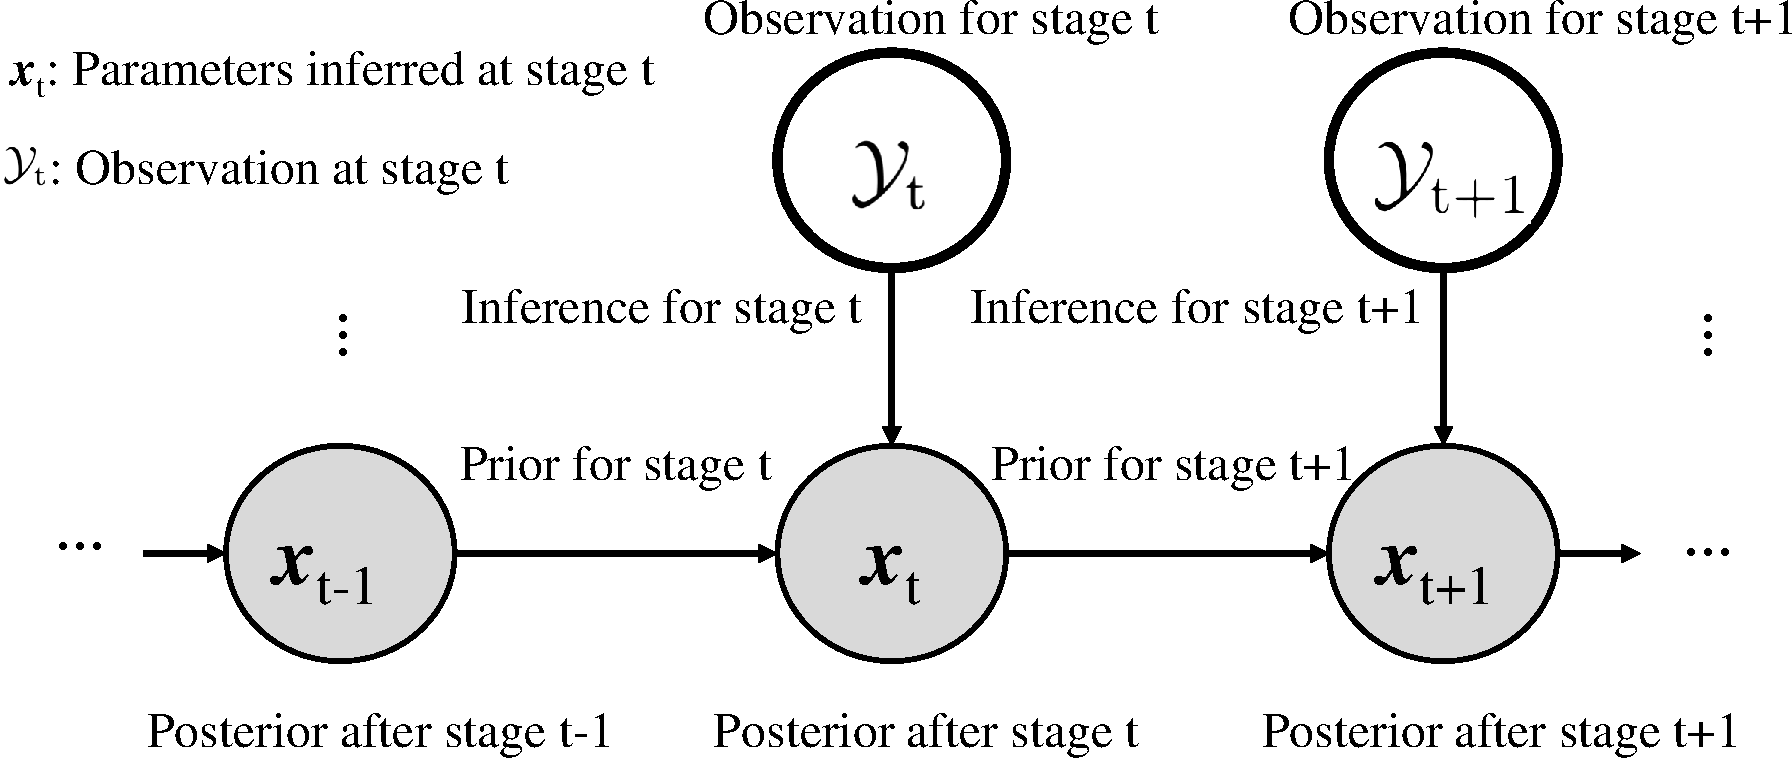
\includegraphics[width = 140mm]{Figures/figures-Sequential_Bayesian.pdf}
    \caption{Sequential Bayesian updating}
    \label{fig: Sequential Bayesian}
\end{figure}
\subsection{Inverse probability transform}
The most straightforward technique for sampling can be \textit{inverse probability transform} from a univariate distribution. As shown in \cref{fig: CDF}, if we can get the \acrfull{CDF}, then we can easily generate samples by computing $\boldsymbol{x}_{t}^{s}$ = CDF($\mathcal{U}$). $\mathcal{U}$ follows uniform distribution $\mathcal{U} \sim U(0,1)$ using a \textit{pseudo random number generator}.
\begin{figure}[H]
    \centering
    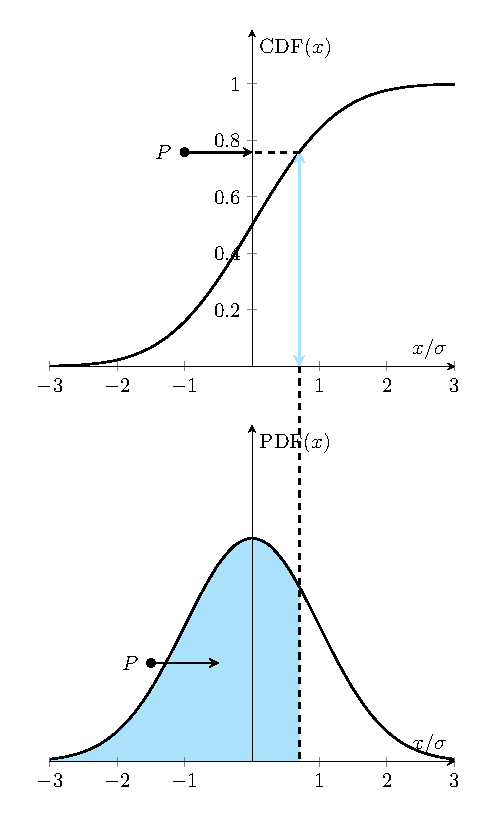
\includegraphics[width = 90mm]{Figures/figure-CDF.pdf}
    \caption{Sampling using an inverse CDF}
    \label{fig: CDF}
\end{figure}
\subsection{Rejection sampling}
In cases where inverse \acrshort{CDF} method is not feasible, a straightforward alternative is to employ \textit{rejection sampling}. We propose a distribution $q(\boldsymbol{x})$ ensuring $Mq(\boldsymbol{x}) \geq \tilde{\pi}(\boldsymbol{x})$, where $M$ is a constant. Here, $\tilde{\pi}(\boldsymbol{x})$ represents unnormalized $\pi(\boldsymbol{x})$ (denoted as $\pi(\boldsymbol{x})$ = $\tilde{\pi}(\boldsymbol{x})/Z$ for some unknown constant $Z$). The function $Mq(\boldsymbol{x})$ serves an upper bound for $\tilde{\pi}$. At time stage $t$, we sample $\boldsymbol{x}_{t}^{s} \sim q(\boldsymbol{x}_{t})$, representing the random selection of a position $\boldsymbol{x}_{t}^{s}$. Subsequently, we sample $u \sim U(0,1)$, representing a random height ($y$ location) under the
upper bound. If $u \geq \frac{\tilde{\pi}(\boldsymbol{x}_{t}^{s})}{Mq(\boldsymbol{x}_{t}^{s})}$, the sample is rejected, otherwise it is accepted. The shaded region in \cref{fig: rejectsampling} shows the acceptance region, and the unshaded region indicates the rejection area.
\begin{figure}[htbp]
    \centering
    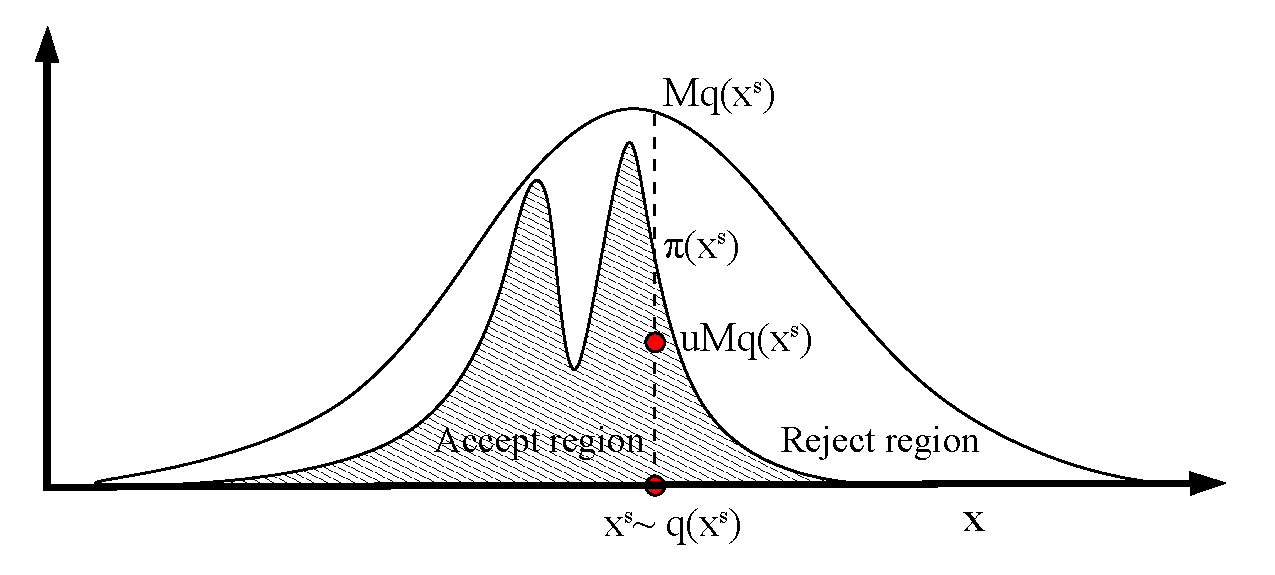
\includegraphics[width = 140mm]{Figures/figure-rejectionsampling.pdf}
\caption{Schematic illustration of \textit{rejection sampling} from \protect\cite{andrieu2003}}
\label{fig: rejectsampling}
\end{figure}
However, in high-dimensional spaces, the vast majority of the space tends to be sparsely populated. Consequently, the likelihood of this method accepting a point can be remarkably low when dealing with multidimensional spaces.
\subsection{Importance sampling}
Now, we introduce a Monte Carlo technique called \textit{importance sampling}, designed for estimating integrals of the following form:
\begin{equation}
    \label{eq: MC_intergral}
    E[f(\boldsymbol{x}_{t})] = \int f(\boldsymbol{x}_{t})\pi(\boldsymbol{x}_{t}) d\boldsymbol{x}_{t}
    \approx \frac{1}{S}\sum_{s=1}^{S} f(\boldsymbol{x}_{t}^{s})
\end{equation}
where $\boldsymbol{x}_{t} \sim \pi(\boldsymbol{x}_{t})$
The idea of \textit{Monte Carlo sampling} is to simply sample $\boldsymbol{x}_{t}$ from the distribution $\pi(\boldsymbol{x}_{t})$. However, when it comes to tricky target $\pi(\boldsymbol{x}_{t})$, the above estimation can be less efficient, meaning it requires huge amounts of samples to ensure the accuracy. In this case, it is more advantageous to sample from a proposed distribution $q(\boldsymbol{x}_{t}) \propto  f(\boldsymbol{x}_{t})\pi(\boldsymbol{x}_{t})$ than directly from $\pi(\boldsymbol{x}_{t})$.

The main concept behind the \textit{importance sampling} is to draw samples at the $t_{th}$ step from a proposed distribution $q(\boldsymbol{x}_{t})$ and adjust the the integral using importance weights to the target distribution. It then uses these samples to estimate the integral as follows:
\begin{equation}
    \label{eq: IS_integral}
    E[f(\boldsymbol{x}_{t})] = \int f(\boldsymbol{x}_{t})\pi(\boldsymbol{x}_{t}) d\boldsymbol{x}_{t} = \int f(\boldsymbol{x}_{t})\frac{\pi(\boldsymbol{x}_{t})}{q(\boldsymbol{x}_{t})}q(\boldsymbol{x}_{t}) d\boldsymbol{x}_{t}
    \approx \frac{1}{S} \sum_{s=1}^{S} f(\boldsymbol{x}_{t}^{s})\frac{\pi(\boldsymbol{x}_{t}^{s})}{q(\boldsymbol{x}_{t}^{s})}
\end{equation}
where $\frac{\pi(\boldsymbol{x}_{t}^{s})}{q(\boldsymbol{x}_{t}^{s})}$ is the importance weight. With a proper proposal distribution $q(\boldsymbol{x}_{t})$, the integral estimation can be close as possible to the true value (improving the approximation means decreasing the variance of estimation $\mathrm{Var}(\boldsymbol{x}_{t}) = \mathbb{E}[{\boldsymbol{x}_{t}}^2] - {\mathbb{E}[\boldsymbol{x}_{t}]}^2$). However, in practice, the choice for the $q(\boldsymbol{x}_{t}^{s})$ is not satisfying. This is a general difficult task, especially in high dimensions.







\subsection{Markov Chain Monte Carlo}
Closed-form expressions for the posterior distribution in \cref{equation Bayes} cannot be derived in general. The exceptions are some linear models with conjugate distributions which were mentioned in \cref{section: Computational methods}. Compared with non-iterative methods above, \acrfull{MCMC} are a category of algorithms enabling the sampling from the posterior by constructing a Markov chain. This process asymptotically converges to the true \acrshort{PDF}.

\acrshort{MCMC} methods were a breakthrough for solving Bayesian inverse problems and since then it has gained tremendous popularity in engineering areas. In a $\href{https://archive.siam.org/pdf/news/637.pdf}{\textit{SIAM News}}$ survey, \acrshort{MCMC} was listed as one of the 10 most important algorithms of the 20th century. Originally developed by statistical mechanics, it is used to construct \textit{Markov chains} to sample a selected \textit{target distribution}. Within the framework of Bayesian updating, this \textit{target distribution} is the posterior in our analysis. Based on the \textit{Markov chains}, every stage depends only on the last previously attained stage. We consider here one discrete \textit{Markov chain} of the type $\mathcal{X}_{t} =\{\boldsymbol{x}_{t}^{1},\cdots,\boldsymbol{x}_{t}^{N_{\mathcal{X}}}\}$, in which $N_{\mathcal{X}}$ is the number of chain iterations, $\mathcal{X}_{t}$ are the samples from sampling process and $t$ is stage number. They start from an arbitrary state $\boldsymbol{x}_{t}^{1} \in \mathcal{D}_{\bm{X}}$ that is updated sequentially based on a \textit{transition kernel}. This kernel is to ensure that \textit{Markov chains} fulfil \textit{detailed balance} condition and are reversible, i.e., that the dynamics of the chains is not affected by the direction of iterative sampling. We omit an in-depth discussion of those properties and refer interest readers to exhaustive resources on the matter in \cite{murphy2012}.

Nowadays, practitioners can choose from a vast of \acrshort{MCMC} algorithms, ranging from the classical \acrfull{MH}, to advanced \textit{Hamiltonian mechanics-inspired samplers}, \textit{transitional MCMC algorithm} and \textit{ensemble algorithms}. In the following, we will present two popular standard \acrshort{MCMC} algorithms that are used in the context of Bayesian inference, but other alternative \acrshort{MCMC} sampling methods can be also easily implemented.
\subsubsection{\acrfull{MH}}
The basic concept of \acrshort{MH} is to choose a proposal distribution $q(\boldsymbol{x}_{t}^{s+1}|\boldsymbol{x}_{t}^{s}),s=1,\cdots,N_{\mathcal{X}}$, between two adjacent samples from the current sample point $\boldsymbol{x}_{t}^{s}$ to the new point $\boldsymbol{x}_{t}^{s+1}$. If we have the first sample $\boldsymbol{x}_{t}^{1}$, we can generate the later samples for any number $N_{\mathcal{X}} > 1$. These samples can be summarized to describe the distribution of inversed parameters $\boldsymbol{x}_{t}$. For any given distribution $\pi(\boldsymbol{x}_{t})$, we define the acceptance function, which is used to decide whether to accept this move, as follows:
\begin{equation}
    \label{eq: accept_ratio_1}    f(\boldsymbol{x}_{t}^{s+1}|\boldsymbol{x}_{t}^{s})=\rm{min}(1,\alpha)
\end{equation}
\begin{equation}
    \label{eq: accept_ratio_2}    
\alpha = {\rm{min}} (1,
\frac{q(\boldsymbol{x}_{t}^{s}|\boldsymbol{x}_{t}^{s+1})  \pi(\boldsymbol{x}_{t}^{s+1}|\mathcal{Y}_{t})}
{q(\boldsymbol{x}_{t}^{s+1}|\boldsymbol{x}_{t}^{s})   \pi(\boldsymbol{x}_{t}^{s}|\mathcal{Y}_{t})} )
\end{equation}
In practice, in order to accept and reject the proposed candidates with probability in \cref{eq: accept_ratio_1} and \cref{eq: accept_ratio_2}, a random variate $u$ is sampled from a uniform distribution $U \sim \mathcal{U}(0,1)$, and compares it to the probability $\alpha$. If $\alpha > 1$, which implies $q(\boldsymbol{x}_{t}^{s}|\boldsymbol{x}_{t}^{s+1})  \pi(\boldsymbol{x}_{t}^{s+1}|\mathcal{Y}_{t})  > q(\boldsymbol{x}_{t}^{s+1}|\boldsymbol{x}_{t}^{s})   \pi(\boldsymbol{x}_{t}^{s}|\mathcal{Y}_{t})$, we accept the candidate sampled point $\boldsymbol{x}_{t}^{(\star)}$ from $q(\boldsymbol{x}_{t}^{s}|\boldsymbol{x}_{t}^{s+1})$. If $\alpha < 1$, we accept the candidate point $\boldsymbol{x}_{t}^{(\star)}$ with probability $\alpha$. If the candidate is accepted, the new sample point $\boldsymbol{x}_{t}^{(\star)}$ is $\boldsymbol{x}_{t}^{s+1}$, otherwise stays the same as $\boldsymbol{x}_{t}^{s}$. A frequently employed proposal distribution is a Gaussian-type distribution centered at $\boldsymbol{x}_{t}^{s}$. The acceptance function can be modified as:
\begin{equation}
    \label{eq: accept_function_Gaussian_distribution}    
f(\boldsymbol{x}_{t}^{s+1}|\boldsymbol{x}_{t}^{s})={\rm{min}}(1,\alpha)={\rm{min}}(1,\frac{q(\boldsymbol{x}_{t}^{s+1})}
{q(\boldsymbol{x}_{t}^{s})})
\end{equation}
\begin{algorithm}
    \caption{\acrlong{MH} algorithm at $t_{th}$ step}
    \label{Algorithm:MH}
    \KwData{ $q(\boldsymbol{x}_{t})$: Proposal distribution; $\pi(\boldsymbol{x}_{t}|\mathcal{Y})$: Target posterior.}
    \KwResult{MCMC samples at $t_{th}$ stage: $\mathcal{X}_{t} = \{\boldsymbol{x}_{t}^{1},\cdots,\boldsymbol{x}_{t}^{N_{\mathcal{X}}}\}$}
    Initialization $\boldsymbol{x}_{t}^{1} \in \mathcal{D}_{\bm{X}}$\; 
    \For{$s \gets 2 \ to  \ N_{\mathcal{X}}$}{
        Sample $\boldsymbol{x}_{t}^{s+1} \sim q(\boldsymbol{x}_{t}^{s+1}|\boldsymbol{x}_{t}^{s})$;\\
        Compute acceptance probability $\alpha$;\\
        Compute $f\left(\boldsymbol{x}_{t}^{s+1}|\boldsymbol{x}_{t}^s\right)=\min{\left(1,\alpha\right)}$;\\
        Sample $u \sim \mathcal{U}\left(0,1\right)$;\\
        Set candidate sample $\boldsymbol{x}_{t}^{(\star)}$ to $\boldsymbol{x}_{t}^{s+1}$ with probability $\alpha$;} 
\end{algorithm}
The process of \acrshort{MH} is shown in \ref{Algorithm:MH}. It is worth mentioning that although the proposal distribution $q(\boldsymbol{x}_{t})$ can be any distribution, the closer it is to the actual target distribution $\pi(\boldsymbol{x}_{t}|\mathcal{Y})$, the more efficient the chain mixture would be. Also, we need to assign an initial position $\boldsymbol{x}_{t}^{1} \in \mathcal{D}_{\bm{X}}$ that is not zero probability. Although the initial position does not affect the convergence of the sampling, a good initial guess would help to accelerate mixing for a Markov chain. With more paralleled $N_{\rm{chain}}$ chains and iterative steps used ($\mathcal{X}_{t} = \{ \mathcal{X}_{t\_1},\cdots,\mathcal{X}_{t\_N_{chain}}\}$), where each chain $\mathcal{X}_{t\_i}$ contains $\{ \boldsymbol{x}_{t\_i}^{1},\cdots,\boldsymbol{x}_{t\_i}^{N_{\mathcal{X}}}\}$, the convergence will be improved accordingly. One schematic representation of the \acrshort{MH} algorithm for sampling can be seen in \cref{fig: MH_example}.
\begin{figure}[htbp]
    \centering
    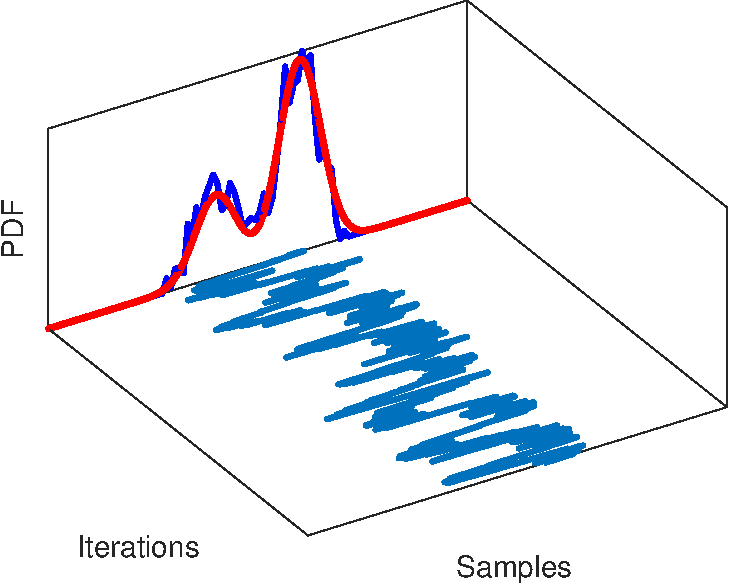
\includegraphics[width = 90mm]{Figures/figure-MCMC_sampling.pdf}
\caption{An schematic figure of the \acrshort{MH} algorithm for sampling from a mixture 1D Gaussian at $t_{th}$ stage}
\label{fig: MH_example}
\end{figure}
\subsubsection{\acrfull{AIES}}
Many \acrshort{MCMC} algorithms perfom poorly when the target (i.e., posterior) distribution $\pi(\boldsymbol{x}_{t}|\mathcal{Y})$ exhibits strong, priorly unknown, inter-parameter correlation. For the \acrshort{MH}, for example, it is challenging to construct a proposal distribution that propose states in the high-probability regions of the parameter space. This results in low acceptance rates which can only be improved by considerable tuning efforts. The \acrshort{AIES} originally presented in \cite{goodman2010} alleviates this problem. Its invariance to affine transformations means that if there exists an affine transformation of the \textit{difficult-to-sample} (by standard \acrshort{MCMC} methods) target distbution to an \textit{easier-to-sample} target distribution, \acrshort{AIES} samples both distributions equally well without explicitly requiring this affine transformation.

The \acrshort{AIES} algorithm presented in \ref{Algorithm:AIES}, simultaneously generates an \textit{ensemble} of $N_{chain}$ \textit{Markov chains} at the $t_{th}$ stage ($\mathcal{X}_{t} = \{ \mathcal{X}_{t\_1},\cdots,\mathcal{X}_{t\_N_{chain}}\}$). Each chain is called a \textit{walker}. At the $\{s_{th}\}_{s \in \{1,\cdots,N_{\mathcal{X}}\}}$ iteration, all \textit{Markov chain states} $\{\boldsymbol{x}_{t\_i}^{s}\}_{i \in \{1,\cdots,N_{chain}\}}$ are updated \textit{walker by walker}. To update the $i_{th}$ \textit{walker}, the algorithm randomly picks a \textit{conjugate walker} from $j \in \{ 1,\cdots,N_{chain}\} \backslash i$, i.e., excluding the current $i_{th}$ walker. The \textit{stretch move} is employed to generate proposals, thereby achieving the affine invariance property. This refers to proposing a new candidate along a straight line between the current walker and the \textit{conjugate walker} with
\begin{equation}
    \label{eq: AIES walker}
\boldsymbol{x}_{t}^{(\star)}
=
\boldsymbol{x}_{t\_i}^{(s)}
+
z \cdot 
(\boldsymbol{x}_{t\_j}^{(\tilde{s})} - \boldsymbol{x}_{t\_i}^{(s)})
\end{equation}
where $\tilde{s} = s +1$ if $j < i$ and $\tilde{t}=s$ otherwise, i.e., it denotes the latest available stage of the $j_{th}$ \textit{walker}. The stretch factor $z$ is randomly drawn from the \acrshort{PDF}
\begin{equation}
    \label{eq: AIES Z}
    p(z|a)= \left\{\begin{matrix}
  \frac{1}{\sqrt{z} (2\sqrt{a} - \frac{2}{\sqrt{a} } )}  & {\rm{if} }\ z \in [1 / a, a]  \\
  0 & {\rm{otherwise} }
\end{matrix}\right.
\end{equation}
which relies on the tuning parameter $a>1$. The candidate sample ${x}_{t}^{(\star)} \in \mathcal{D}_{\boldsymbol{X}} \subseteq \mathbb{R}^{M}$ is then accepted as the new location of the $i_{th}$ walker with probability:
\begin{equation}
    \label{eq: AIES acceptance probability}
    \alpha = {\rm{min}}
(1,
z^{M-1} 
\frac{\pi({x}_{t}^{(\star)}|\mathcal{Y})}
{\pi({x}_{t\_{i}}^{(s)}|\mathcal{Y})} 
)
\end{equation}
This is repeated for all $N_{chain}$ walkers in the ensemble. The resulting chains fulfil the \textit{detailed balanced condition}. A practical advantage of the \acrshort{AIES} algorithm is that it only has a single scalar tuning parameter $a$, which is often set to $a=2$ \citep{UQdoc}.
\begin{algorithm}    
    \caption{\acrlong{AIES} algorithm at $t_{th}$ step}
    \label{Algorithm:AIES}
    \KwData{$\pi(\boldsymbol{x}_{t}|\mathcal{Y})$: Target posterior; tuning parameter $a$}
    \KwResult{MCMC samples at $t_{th}$ stage: $\mathcal{X}_{t} = \{ \mathcal{X}_{t\_1},\cdots,\mathcal{X}_{t\_N_{chain}}\}$), with $\mathcal{X}_{t\_i}=\{ \boldsymbol{x}_{t\_i}^{1},\cdots,\boldsymbol{x}_{t\_i}^{N_{\mathcal{X}}}\}$}
    Initialization $N_{chain}$ samples $\{  \boldsymbol{x}_{t\_1}^{1},\cdots,\boldsymbol{x}_{t\_{N_{chain}}}^{1}\}$, with $\boldsymbol{x}_{t\_i}^{1} \in \mathcal{D}_{\boldsymbol{X}}$\
    
    \For{$s \gets 2 \ to  \ N_{\mathcal{X}}$}{
        \For{$ i \in \{ 1,\cdots,N_{chain}\}$}{
            Pick random $j$ from $\{ 1,\cdots,N_{chain}\} \backslash i$;\\
            Propose ${x}_{t}^{(\star)}$ with \cref{eq: AIES walker};\\
            Set $\boldsymbol{x}_{t\_i}^{s} = {x}_{t}^{(\star)}$ with probability $\alpha$ (see \cref{eq: AIES acceptance probability});
        }        
        } 
\end{algorithm}



\subsection{Sequential Monte Carlo}

Like \acrshort{MCMC}, \acrfull{SMC}, is another popular sampling method for a dynamic model. The parameters $\boldsymbol{{x}_{t}}$ which we are interested can be linked with the observations $\mathcal{Y}_{t}$ in a time series way:
\begin{equation}
\label{eq: Bayesian filtering}
\begin{aligned}
   & \boldsymbol{{x}_{t}}  =g(\boldsymbol{{x}_{t-1}}) + \boldsymbol{v} \ \   \ &\rm{(state  \ equation)}\\    
     &\mathcal{Y}_{t}=m(\boldsymbol{{x}_{t}}) + \boldsymbol{w} \ \ \ \ \ &\rm{(observation \  equation)}
\end{aligned}
\end{equation}
which stands for the prediction step and correction step, respectively.
$g(\cdot)$ and $m(\cdot)$ denote \textit{transition equation} and \textit{emission equation}, respectively. These functions can be either linear or nonlinear. $\boldsymbol{v}$ and $\boldsymbol{w}$ are independent random variables (or vectors) that denote process noise and observation noise, respectively.


In this setting, we only focus on nonlinear non-Gaussian dynamic model, often referred to as a \textit{particle filter}. The feature of the non-linearity is used to relax the constraints at some simplified models (i.e., Kalman filter (KF) or Unscented Kalman filter (UKF), etc.). \acrshort{SMC}, a sequential Bayesian technique, involves getting a population of non-correlated particles where each sample denotes to a potential parameter set. Subsequently, these particles undergo filtering to approximate the final distribution in a manner that aligns with the posterior distribution $\pi(\boldsymbol{x}_{t}|\mathcal{Y})$. The filtering process usually encompasses several steps: initial samples, reweighting and resampling, which are sequentially applied while new observations $\mathcal{Y}_{t}$ are added. There are different flavours of \textit{particle filter}. For book-length treatment, see \cite{murphy2012}. Due to space limitation, we will only present two standard \acrshort{SMC} algorithms that are used in the context of Bayesian inference, but other effective \textit{particle filter} methods can be also easily implemented.


\subsubsection{Sequential importance sampling}
The concept is to estimate the belief state of the trajectory stage by utilizing a weighted set of particles:
\begin{equation}
    \label{eq: PF-SIS}
\pi(\boldsymbol{x}_{1:t}|\mathcal{Y}_{1:t})
\approx 
\sum_{s=1}^{S} 
\tilde{w}_{t}^{s}
\delta_{\boldsymbol{x}_{1:t}^{s}}(\boldsymbol{x}_{1:t})
\end{equation}
\begin{equation}
    \label{eq: PF-SIS-Normalized_weight}
\tilde{w}_t^s=\frac{w_t^s}{\sum_{s=1}^{S}{(w_t^s)}}
\end{equation}
where $\tilde{w}_{t}^{s}$ represents the normalised weight of sample $s = \{1,\cdots,N\}$ at time $t$ and  $\delta$ denotes the \textit{Dirac delta function}. Utilizing this representation, we can straightforwardly calculate the marginal distribution over the most recent state,$\pi(\boldsymbol{x}_{t}|\mathcal{Y}_{1:t})$, by simply disregarding the preceding segments of the trajectory $\boldsymbol{x}_{1:t}$.

We revise this belief state through importance sampling. If the proposal takes the form $q(\boldsymbol{x}_{1:t}|\mathcal{Y}_{1:t})$, we can recursively express the numerator as follows:
\begin{equation}
    \label{eq: PF-recursive}
    \pi(\boldsymbol{x}_{1:t}|\mathcal{Y}_{1:t})
    \propto 
    \pi(\mathcal{Y}_{t}|\boldsymbol{x}_{t})
    \pi(\boldsymbol{x}_{t}|\boldsymbol{x}_{t-1})
    \pi(\boldsymbol{x}_{t-1}|\mathcal{Y}_{t-1})
\end{equation}
where we have employed the customary Markov assumptions. Our focus will be on proposal densities in the following form:
\begin{equation}
    \label{eq: PF-recursive_2}
\pi(\boldsymbol{x}_{1:t}|\mathcal{Y}_{1:t})
=
\pi(\boldsymbol{x}_{t}|\boldsymbol{x}_{1:t-1},\mathcal{Y}_{1:t})
\pi(\boldsymbol{x}_{1:t-1}|\mathcal{Y}_{1:t-1})
\end{equation}
Next, incorporating the new state $\boldsymbol{x}_{t}$ at the end, we assume the necessity to retain only the most recent portion of the trajectory and observation sequence, rather than the entire history $1:t$ for simplicity. In such a scenario, the weight takes the following form:
\begin{equation}
    \label{eq: PF-modified_weight}
    w_{t}^{s}
    \propto 
    w_{t-1}^{s}
    \frac{\pi(\mathcal{Y}_{t}|\boldsymbol{x}_{t}^{s})     \pi(\boldsymbol{x}_{t}^{s}|\boldsymbol{x}_{t-1}^{s})}
    {q(\boldsymbol{x}_{t}^{s}|\boldsymbol{x}_{t-1}^{s},\mathcal{Y}_{t})} 
\end{equation}
Hence we can approximate the posterior $\pi(\boldsymbol{x}_{t}|\mathcal{Y}_{1:t})$ filtered density using \cref{eq: PF-SIS_simplified}
\begin{equation}
    \label{eq: PF-SIS_simplified}
    \pi(\boldsymbol{x}_{t}|\mathcal{Y}_{1:t})
    \approx 
    \sum_{s=1}^{S} 
    \tilde{w}_{t}^{s}
    \delta_{\boldsymbol{x}_{t}^{s}}(\boldsymbol{x}_{t})
\end{equation}
As $S \rightarrow \infty$, it can be demonstrated that this converges to the true posterior. All initial particles share the same weight values and can be uniformly sampled using \textit{Latin hypercube sampling} within feasible ranges of parameter values. The whole \acrshort{SIS} without resampling process is shown in \cref{fig: PF-SIS} and \acrshort{SIS} algorithm is presented in \ref{Algorithm:SIS}.
\begin{figure}[htbp]
    \centering
    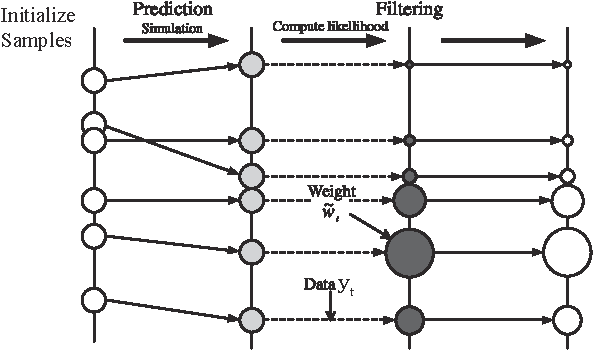
\includegraphics[width = 140mm]{Figures/figure-PF-SIS.pdf}
\caption{Particle filtering using \acrshort{SIS} adapted from \protect\cite{nguyen2016}}
\label{fig: PF-SIS}
\end{figure}
\begin{algorithm}[htbp] 
    \caption{\acrlong{SIS} algorithm at $t_{th}$ step}
    \label{Algorithm:SIS}
    \KwData{Samples $\boldsymbol{x}_{t-1}^{s}$ with weights $w_{t-1}^{s},\ s = \{1,\cdots,N\}$; observation $\mathcal{Y}_{t}$ at $t_{th}$ stage}
    \KwResult{SMC samples with normalized weights $\tilde{w}_{t}^{s}$ at $t_{th}$ stage: $\boldsymbol{x}_{t}^{(\star)} = \mathcal{X}_{t} = \{\boldsymbol{x}_{t}^{1},\cdots,\boldsymbol{x}_{t}^{N} \}$)}
    \For{$s \gets 1 \ to  \ N$}{
            Sample from proposal distribution $\boldsymbol{x}_{t}^{s} \sim q(\boldsymbol{x}_{t}^{s}|\boldsymbol{x}_{t-1}^{s},\mathcal{Y}_{t})$;\\
            Compute weight using \cref{eq: PF-modified_weight};
        } 
        Normalized weights;
\end{algorithm}

\subsubsection{Sequential importance sampling and resampling}
The fundamental \acrshort{SIS} algorithm encounters challenges after a few steps due to the fact that the majority of the particles will possess negligible weight. This issue is referred to as the \textit{degeneracy problem}, particularly prevalent when sampling in a high-dimensional space. We can measure the degree of degeneracy using the \textit{effective sample size}, defined as:
\begin{equation}
    \label{eq: SISR_Seff}
\hat{S}_{eff}=
\frac{1}{\sum_{s=1}^{S} 
(w_{t}^{s})^2
} 
\end{equation}
If the variance of the weights is substantial, we are essentially allocating resources to update particles with low weight, which contribute minimally to our posterior estimate. An effective approach to address the degeneracy problem involves introducing a resampling step. This enhancement to the basic \acrshort{SIS} algorithm monitors the \textit{effective sample size}. Whenever it falls below a threshold $S_{min}$, particles with low weight are eliminated, and replicates of the surviving particles are generated. This procedure is illustrated in \cref{fig: PF-SISR} and the comprehensive \acrshort{SISR} algorithm is outlined in \ref{Algorithm:SISR}. In this case, $\boldsymbol{x}_{t}^{(\star)} \neq \mathcal{X}_{t}$ comes from fact that the resampling process discards low weighted particles.


\begin{figure}[H]
    \centering
    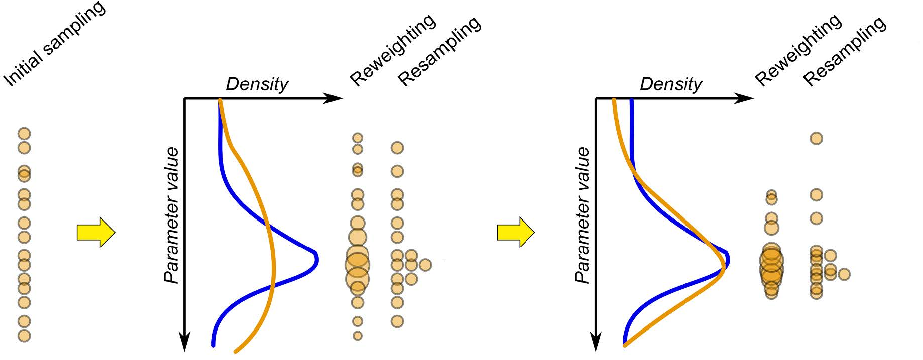
\includegraphics[width = 140mm]{Figures/figure-PF-SISR.pdf}
\caption{Principle of \acrshort{SISR} algorithm adapted from \protect\cite{speich2021}}
\label{fig: PF-SISR}
\end{figure}

\begin{algorithm}    
    \caption{\acrlong{SISR} algorithm at $t_{th}$ step}
    \label{Algorithm:SISR}
    \KwData{Samples $\boldsymbol{x}_{t-1}^{s}$ with weights $w_{t-1}^{s},\ s = \{1,\cdots,N\}$; observation $\mathcal{Y}_{t}$ at $t_{th}$ stage}
    \KwResult{SMC samples with normalized weights $\tilde{w}_{t}^{s}$ at $t_{th}$ stage: $\boldsymbol{x}_{t}^{(\star)} = \{\boldsymbol{x}_{t}^{1},\cdots,\boldsymbol{x}_{t}^{N} \}$)}
    \For{$s \gets 1 \ to  \ N$}{
            Sample from proposal distribution $\boldsymbol{x}_{t}^{s} \sim q(\boldsymbol{x}_{t}^{s}|\boldsymbol{x}_{t-1}^{s},\mathcal{Y}_{t})$;\\
            Compute weight using \cref{eq: PF-modified_weight};
        } 
        Normalized weights;\\
        Calculate degeneracy measure using \cref{eq: SISR_Seff};\\
        \If{$\hat{S}_{eff} < S$}{
        Resample;\\        
        }
\end{algorithm}



\section{Choices for sampling methods}

In a continuous Bayesian calibration process, \acrshort{MCMC} and \acrshort{SMC} are two prevalent sampling methods. They are differed based on different sampling principles. \acrshort{MCMC}-derived uncertain variables are iteratively constructed based on \textit{random walk} and outperforms in high dimensions, while \acrshort{SMC}-derived uncertain variables are represented by updating weights on the particles and yields faster inference results. As shown in \cref{fig: PFvsMCMC_1,fig: PFvsMCMC_2}, both methods demonstrates their effectiveness in updating parameters in a two dimensional space example.

\begin{figure}
\centering
\begin{subfigure}[htbp]{1.0\textwidth}
   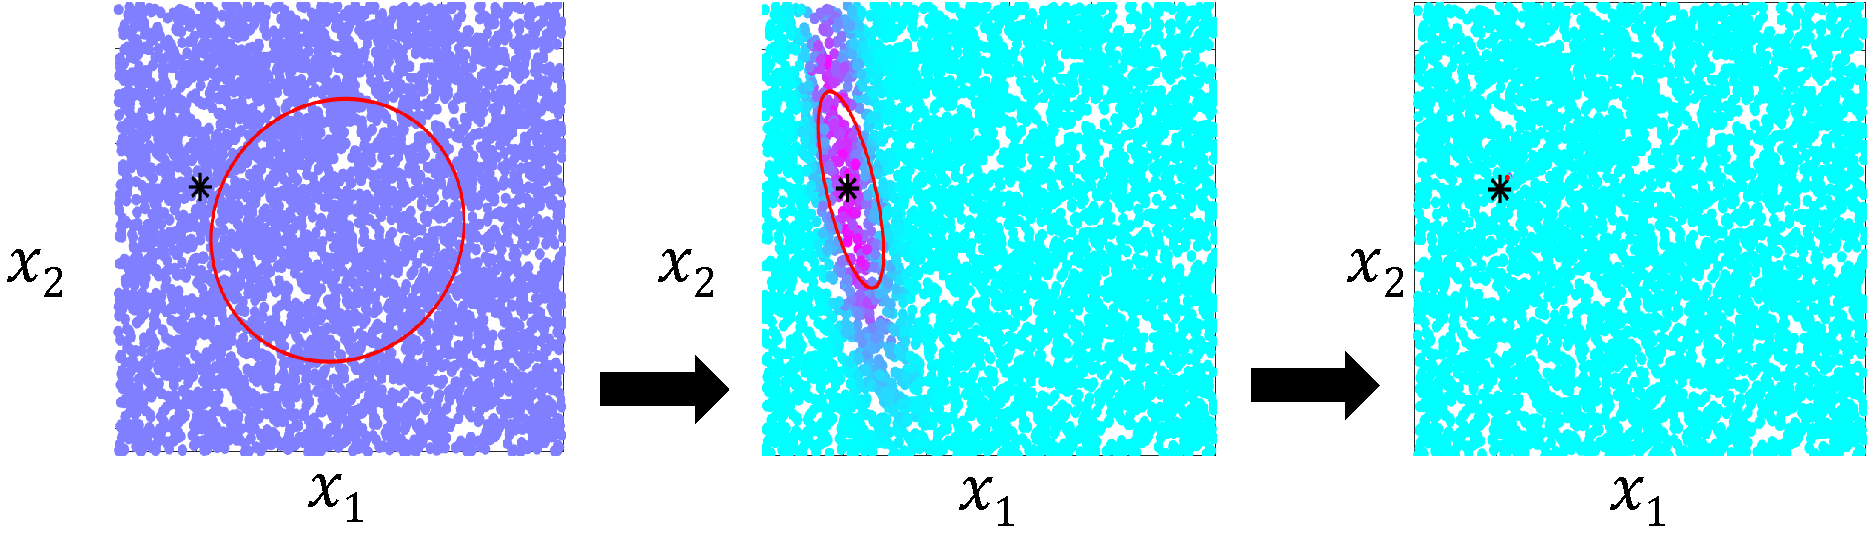
\includegraphics[width=140mm]{Figures/figure-PFvsMCMC-SIS.pdf}
   \caption{Particle filter with \acrlong{SIS}}
   \label{fig: PFvsMCMC_1} 
\end{subfigure}

\begin{subfigure}[htbp]{1.0\textwidth}
   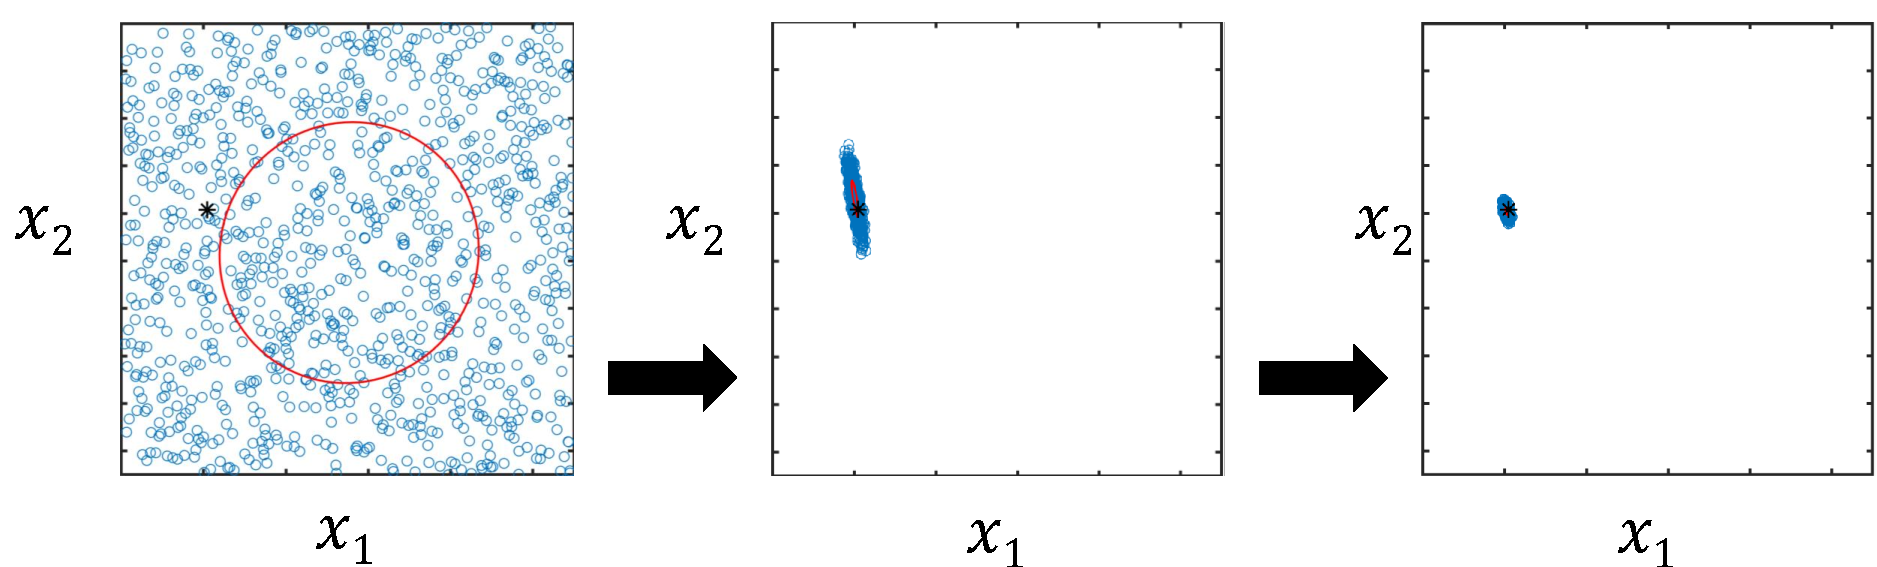
\includegraphics[width=140mm]{Figures/figure-PFvsMCMCAIES.pdf}
   \caption{\acrlong{MCMC} using \acrlong{AIES}}
   \label{fig: PFvsMCMC_2}
\end{subfigure}

\caption[Two sampling method]{\acrshort{SMC} and \acrshort{MCMC} in a two-dimensional example}
\end{figure}

SMC, with its non-iterative nature, offered the advantage of parallel processing, significantly enhancing computational efficiency. This attribute makes \acrshort{SMC} a favorable option when quick results are imperative. However, \textit{particle filter} doesnot work well in high dimensional spaces \citep{murphy2012}. Instead, \acrshort{MCMC}, with its random walk approach, showcased its proficiency in exploring high-dimensional parameter spaces, making it a suitable choice for complex and multifaceted problems. Therefore, the choice between these methods should be guided by the specific needs and priorities of the analysis, whether precision or computational efficiency takes precedence. Since geotechnical engineering are naturally in high dimensional space, this thesis adopts \acrshort{MCMC} during the sequential Bayesian calibration for the next sampling analysis.


